\section{Einführung}

\begin{frame}{Motivation}
    \mycomment{
        Wenn man mit TikZ in \LaTeX\ Grafiken erstellt, möchte man diese in verschiedenen Formaten einbinden, und zwar ohne Copy-Paste.
    }
    \mytext{
    \begin{itemize}
        \item Iterative Grafiken mit Tikz
        \item Erstellen einheitlicher Folien
        \item Möglichkeit von iterativem Bildaufbau
        \item Simultane Ausgabe als Skript
    \end{itemize}
    }
\end{frame}

\section{Beispiel}


\begin{frame}{Beispiel: IS-LM}
    \mycomment{Zur Veranschaulichung entwickeln wir nun eine Grafik. Erst einmal eine Kurve namens $IS$.}
    \showmytikz[1]{shared/tikz/tikz-islm}
    
\end{frame}

\begin{frame}{Beispiel: IS-LM}
    \mycomment{Die Kurve $LM$ schneidet.}
    \showmytikz[1,3]{shared/tikz/tikz-islm}
\end{frame}


\section{Grundidee}

\begin{frame}[fragile]{Arbeitsablauf}
    
    \cprotect\mytext{
    \begin{verbatim}
        
\documentclass{standalone}
\usepackage{tikz}
\begin{document}
    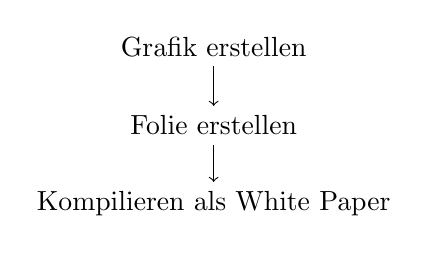
\begin{tikzpicture}
        \node (A) at (0,0) {Grafik erstellen};
        \node (B) at (0,-1) {Folie erstellen};
        \node (C) at (0,-2) {Kompilieren als White Paper};
        \draw[->] (A) -- (B);
        \draw[->] (B) -- (C);
    \end{tikzpicture}
\end{document}
    \end{verbatim}
    }
    \mycomment{Erst werden die Grafiken mit TikZ erstellt - hier ein Minimalbeispiel ohne schrittweise Entwicklung.}
\end{frame}

\begin{frame}[fragile]{Arbeitsablauf}
    
    \cprotect\mytext{
    

Die Einbindung erfolgt mit

    \begin{verbatim}
\showmytikz[]{../shared/tikz/tikz-slideworkflow}
    \end{verbatim}
    
    \showmytikz[]{../shared/tikz/tikz-slideworkflow}
    }
    \cprotect\mycomment{
    Falls nötig, wird die Grafik automatisch verkleinert. 
    }
\end{frame}

\section{Verwendung}

\begin{frame}{Erstellen von Frames}
    \mycomment{
    Dieses Paket stellt \LaTeX-code zur Verfügung, mit dem sich Vorlesungen und Skripte aufbauen lassen - idealerweise besser als mit jedem anderen Tool.
    }
    \mytext{
    \begin{itemize}
        \item Grafiken mit TikZ, die sich nacheinander aufbauen
        \item Grafiken stehen immer an derselben Stelle auf allen Folien
        \item Folien und White Cover Version mit identischem Inhalt
        \item Schlankes HSB-Design
    \end{itemize}
    }
\end{frame}

\begin{frame}[fragile]{Erstellen von Frames}
    \mycomment{
    Dazu werden Folien in \texttt{beamer}  erstellt, die Inhalte jedoch jeweils in besonderen Umgebungen eingebunden.
    }
    
    \cprotect\mytext{
    
    \scriptsize
    
    \begin{verbatim}
%\begin{frame}{Motivation}
    \mycomment{
        Dieses Paket stellt \LaTeX-code zur Verfügung, 
        mit dem sich Vorlesungen und Skripte aufbauen lassen - 
        idealerweise besser als mit jedem anderen Tool.
    }
    \mytext{
        \begin{itemize}
            \item Grafiken mit TikZ, die sich nacheinander aufbauen
            \item Grafiken stehen immer an derselben Stelle auf allen Folien
            \item Folien und White Cover Version mit identischem Inhalt
            \item Schlankes HSB-Design
        \end{itemize}
    }
%\end{frame} 
    \end{verbatim}
    }
\end{frame}

\begin{frame}[fragile]{Commands}
    \mytext{
    Text und Tabellen können ineinander sein; dann erscheint der Text nur in der Breite des Haupt-Textfeldes, während die Tabelle so breit sein kann wie sie möchte.

    Der Brottext hier schiebt die Tabelle nach unten.
    
        \mytable{
            \begin{tabular}{lll}
                \toprule
                 command             & \texttt{beamer} & \texttt{scrartcl} \\
                \midrule
                 \texttt{mytext}    & Text (Stichpunkte) im Hauptfeld & Brottext \\
                 \texttt{mycomment} & Text im Kommentarfeld & Brottext \\
                 \texttt{mytable} & (Tabelle), ganze Breite & Tabellenumgebung \\
                 \midrule
                 \texttt{showmytikz} & Grafik im Hauptfeld & Figure-Umgebung \\
                 \texttt{showmybitmap} & Grafik im Hauptfeld & Figure-Umgebung \\
                 \bottomrule
            \end{tabular}    
        }
    }
    \mycomment{
        Ein Kommentar macht dann meist keinen Sinn, da das Kommentarfeld Gefahr läuft, sich mit der Tabelle zu überlappen.
    
        Das passiert hier nur deswegen nicht, weil oberhalb der Tabelle ein Text im Haupfeld steht; dieses schiebt die Tabelle nach unten. Jedenfalls ist hier Vorsicht geboten und es empfiehlt sich, Tabellen auf jeweils ganz eigenen Folien alleine stehen zu haben.
    }
    
\end{frame}

\begin{frame}{Titel im Whitepaper}
    \mytext{
    Im Whitepaper wird immer nur dann ein neues (unnumeriertes) Unterkapitel begonnen und eine Überschrift ausgegeben, wenn die Folgefolie einen anderen Titel hat.

    Daher ist sinnvoll, den Inhalt auf möglichst viele Frames / Folien aufzuteilen.
    }
    \mycomment{
    Ansonsten gilt: im Whitepaper werden Tabellen und Grafiken numeriert und referenziert, was in der \texttt{beamer}-Version nicht stattfindet. Dazu werden ein paar eigene Zähler eingeführt.

    Möglichst jede Folie sollte einen Kommentar (wie diesen) beinhalten, zumindest alle mit Grafiken.
    }
\end{frame}

\begin{frame}{Titel im Whitepaper}
    \mytext{
    So steht dieser Inhalt auf einer neuen Folie, aber unter derselben Überschrift. Im Whitepaper wird kein neuer Titel vor "`So steht"' ausgegeben.
    }
    \mycomment{
    Auf den Folien erscheinen die Inhalte von \texttt{mytext} und \texttt{mycomment} an verschiedenen Orten und in unterschiedlicher Schrift. Im Whitepaper erscheinen sie beide als Brottext. Dabei lässt sich durch unterschiedliche Reihung beider eine Reihenfolge im Whitepaper vorgeben; für die Folien ist die Reihung beider ohne Belang.

    Es empfiehlt sich aber generell, im \texttt{mycomment} ganze Sätze zu verwenden. Jede Folie sollte so einen Text aufweisen. 
    }
\end{frame}

\begin{frame}[fragile]{Grafiken mit TikZ}

    \cprotect\mycomment{
    Diese Umgebung ruft die TikZ-Datei auf mittels  
    \verb|\input{mytikz.tex}|. Je nach Dokumentenklasse wird sie auf der Folie links oder im Whitepaper in einer \verb|figure|-Umgebung ausgegeben.
    }
    \cprotect\mytext{
    Zum Einbinden von TikZ-Grafiken gibt es den Befehl
    
    \begin{verbatim}
        \showmytikz[steps]{mytikz.tex}
    \end{verbatim}

    Wobei \verb|steps| Zahlen 1,2,3 usw. sein dürfen. 
    }
\end{frame}

\begin{frame}[fragile]{Grafiken mit TikZ}

    \cprotect\mytext{
    Dabei lassen sich einzelne Teile anzeigen mittels folgedem Befehl in den TikZ-Grafiken:

    \begin{verbatim}
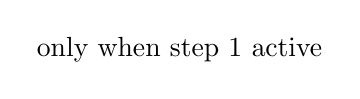
\begin{tikzpicture}
...
    \ifstep{1}{
        \node {only when step 1 active};
    }
...
\end{tikzpicture}
    \end{verbatim}
    }
    
    \cprotect\mycomment{
        Ergänzend gibt es \verb|\ifsteponly{1}{2}{}|, was nur dann erscheint, wenn 1 aktiv und 2 \textit{nicht} aktiv ist.

        Diese Befehle lassen sich verschränken.
    }
    
\end{frame}

\begin{frame}[fragile]{Grafiken mit TikZ}

    \cprotect\mytext{
        Der Schalter mit den Steps ist im Paket voreingestellt definiert. 
        
        Möchte man die Grafiken als Standalone einzeln kompilieren, so muss man in der Präambel der \verb|standalone|-Datei hinzufügen:

        \begin{verbatim}
%% Show/hide steps for standalone work — edit this:
\makeatletter
\AtBeginDocument{\@buildstepset{1,2,3,4,5}}
\makeatother
        \end{verbatim}      
    
    }

    \cprotect\mycomment{
        Dabei bewährt es sich, die Schritte in jeweils eigene \verb|scope|-Umgebungen zu wrappen, um sie beispielsweise farblich voneinander abzusetzen.
    }
    
\end{frame}

\begin{frame}[fragile]{Grafiken mit TikZ}

    \cprotect\mytext{
    \begin{verbatim}
\documentclass{standalone}
\usepackage{tikz}
% \usepackage{hsbcommon} % for colours etc.
\makeatletter\AtBeginDocument{\@buildstepset{1,2,3,4,5}}\makeatother
\begin{document}

\begin{tikzpicture}
...
    \ifstep{1}{
        \begin{scope}[color=red]
            \node {only when step 1 active};
        \end{scope}
    }
...
\end{tikzpicture}
    \end{verbatim}
    }
    
    \cprotect\mycomment{
        Hier sind durch die 4. Zeile die Schritte  $1,2,3,4,5$  aktiviert. Benutzt man \verb|hsbcommon|, so ist die Zeile nicht zwingend notwendig; sie ist aber sehr nützlich bei der Entwicklung dieser Grafiken.
    }
    
\end{frame}

\begin{frame}[fragile]{Bitmaps einbinden}
    
    \cprotect\mytext{
    Und dann gibt es noch die Möglichkeit, Rastergrafiken einzubinden. Der Befehl lautet:
    \begin{verbatim}
        \showmybitmap{shared/bitmaps/ce.png}        
    \end{verbatim}
    
    \showmybitmap{shared/bitmaps/ce.png}
    }
    \mycomment{Auch dieser Befehl kann innerhalb von \texttt{mytext} stehen, falls man vor oder unter der Grafik noch etwas Text anzeigen möchte. Der Befehl ersetzt \texttt{includegraphics} nur, um im Whitepaper-Modus eine Abbildungsumgebung zu erzeugen.}
\end{frame}
    

\begin{frame}[plain]{}
    \begin{center}
    \Large
    ~\par\vspace{3cm}
    Thank you!
    \end{center}
\end{frame}

\begin{frame}[allowframebreaks]{Literature and Links}
   \nocite{*}
    \printbibliography
\end{frame}
